\subsection{Principal component analysis}
\label{sec:pca}

PCA is needed to handle the multicollinearity of the predictors before they
enter the models: \texttt{NO} and \texttt{NOX} correlate at 0.95. The
expected outcome is a set of principal components with names that are
interpretable in context, together with the structure of their loadings. The
procedure is applied to the station-day data. The categorical variables
(\texttt{tipo\_dia}, \texttt{temporada}, \texttt{festivo}, \texttt{zona}) are
excluded, as are the variables derived from \texttt{O3} and the exceedance
indicators: these are the response, and using them would leak information,
building components that contain what is meant to be predicted. Of the 16
continuous daily variables, \texttt{PM2.5} is also excluded, because station
\texttt{NE3} does not measure it and listwise deletion would remove that
station entirely; its signal is largely carried by \texttt{PM10} ($r=0.70$).
PCA therefore runs on 15 predictors.

It is fitted on 2021--2024 only and applied to 2025 (\cref{sec:modelacion}).

The eigenvalues are computed and the scree plot is built
(\cref{fig:scree_pca}); the number of components to retain is set by the
elbow method. The curvature places the cut at the third principal component.

The loadings are the product of the eigenvectors and the square root of the
corresponding eigenvalues, so they are interpreted as the correlation between
the variables and the components (\cref{tab:pca-cargas}).

The first component has high loadings on \texttt{NOX}, \texttt{NO2},
\texttt{NO} and \texttt{PM10}, and a negative loading on \texttt{WSR\_min}
($-0.48$). These variables are mainly the substances that take part in the
chemical reactions that form ozone, whose main source is the burning of
fossil fuels, while wind speed (with a negative loading) acts as dispersion;
for this reason \texttt{PC1} is named \textit{primary combustion load}.

\texttt{PC2} has high negative loadings on relative humidity and high
positive loadings on solar radiation and temperature. These variables are
related: as temperature rises, relative humidity falls, since warm air can
hold more water vapor, and sunnier, drier days increase ozone production.
This component is \textit{photochemical forcing}.

The third component gathers the conditions that affect the stagnation of
pollutants: higher pressure increases stagnation, and higher wind speed
reduces it. This component is \textit{atmospheric stagnation}
(\cref{fig:pca_biplot}).

The three components account for 55.9\,\% of the variance of the 15
predictors. The benchmark for that figure is not 100\,\% but what three
components would produce on independent variables: with $p = 15$ each
eigenvalue would equal 1 and three would account for 20\,\%. The retained
eigenvalues are 3.92, 2.97 and 1.50, 2.8 times the null. The correlation
between \texttt{NO} and \texttt{NOX} that motivated the analysis is absorbed
into \texttt{PC1}, and the three coordinates inherited by the subsequent
models are orthogonal by construction. The mean 2025 scores are not zero
(\texttt{PC1} $-0.39$, \texttt{PC3} $+0.35$): 2025 has less primary load and
more stagnation than the 2021--2024 average, the year effect of
\cref{sec:modelacion}, not a fitting error.

\begin{figure}[t]
  \centering
  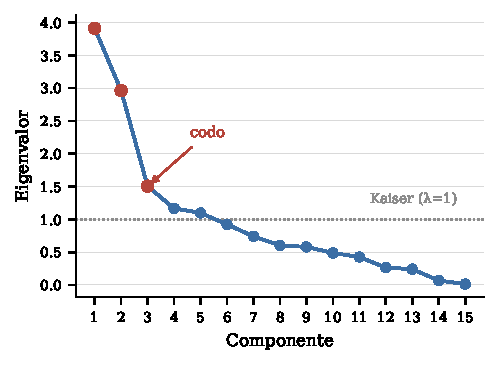
\includegraphics[width = \linewidth]{pca_scree.pdf}
  \caption{Variance explained by each component. The largest drop occurs at
    the third component; beyond it the gain is marginal.}
  \label{fig:scree_pca}
\end{figure}

\begin{table}[ht]
  \centering
  \caption{Dominant loadings of the retained components, with the variance
    explained by each.}
  \label{tab:pca-cargas}
  \begin{tabular}{lr}
    \toprule
    Component and variable & Loading \\
    \midrule
    \multicolumn{2}{l}{\emph{Primary combustion load} (26.1\,\%)} \\
    \quad \texttt{NOX}      & 0.88 \\
    \quad \texttt{NO}       & 0.82 \\
    \quad \texttt{NO2}      & 0.81 \\
    \quad \texttt{PM10}     & 0.66 \\
    \quad \texttt{WSR\_min} & $-0.48$ \\
    \midrule
    \multicolumn{2}{l}{\emph{Photochemical forcing} (19.8\,\%)} \\
    \quad \texttt{RH\_min\_diurna} & $-0.77$ \\
    \quad \texttt{TOUT\_max}       & 0.72 \\
    \quad \texttt{RH\_media}       & $-0.70$ \\
    \quad \texttt{SR\_acum}        & 0.64 \\
    \quad \texttt{WSR\_media}      & 0.61 \\
    \midrule
    \multicolumn{2}{l}{\emph{Atmospheric stagnation} (10.0\,\%)} \\
    \quad \texttt{WSR\_min}        & $-0.50$ \\
    \quad \texttt{viento\_u\_media} & 0.48 \\
    \quad \texttt{WSR\_media}      & $-0.41$ \\
    \quad \texttt{PRS\_media}      & 0.40 \\
    \quad \texttt{RH\_min\_diurna} & $-0.37$ \\
    \bottomrule
  \end{tabular}
\end{table}

\begin{figure}[t]
  \centering
  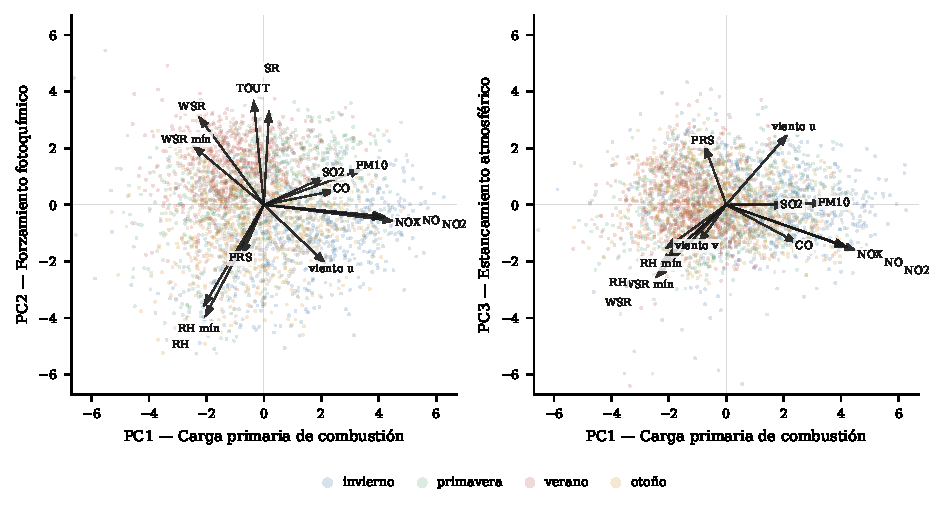
\includegraphics[width = \linewidth]{pca_biplot.pdf}
  \caption{Biplot of the retained axes. Points: subsample of 3,000 training
    observations, colored by season. Arrows: loadings scaled to the frame.
    Abbreviated names: \texttt{TOUT} and \texttt{SR} are the daily maximum
    and total; \texttt{NO}, \texttt{NO2}, \texttt{NOX} and \texttt{CO} are
    the 06--09 h window; the rest are daily means, except \texttt{WSR} min
    and \texttt{RH} min.}
  \label{fig:pca_biplot}
\end{figure}
